\section{Theoretische Grundlagen}

\subsection{Supraleitung}

Supraleiter sind Materialien mit der Eigenschaft, dass sie widerstandslos Strom leiten können, wenn sie unter eine bestimmte Temperatur (genannt: kritische Temperatur $T_c$) gekühlt werden. Sie verhalten sich wie ideale Diamagneten, erzeugen also ein durch die inneren Ströme induziertes Magnetfeld, welches Magnetfelder von außen komplett kompensieren und somit sind sie im Inneren komplett feldfrei (Meißner-Ochsenfeld-Effekt). Je nach Verhalten in einem externen Magnetfeld unterscheidet man 2 Arten von Supraleiter:

\paragraph{Typ I: }  Das Magnetfeld wird bis auf eine dünne Schicht (exponentieller Abfall von außen, genannt \emph{London'sche Eindringtiefe}) an der Oberfläche des Leiters komplett aus dem Inneren verdrängt. Erreicht das Magnetfeld einen kritischen Wert $B_c$, so wird der Supraleiter wieder normalleitend. Die kritischen Temperaturen liegen beim Typ I bei maximal $23,2K$ ($Nb_3Ge$).

\paragraph{Typ II: } Supraleiter vom Typ II, auch Hochtemperatursupraleiter genannt, besitzen zwei kritische Magnetfeldstärken $B_{c1}$ und $B_{c2}$ (mit $B_{c1} < B_{c2}$). Unter dem kritischen Feld $B_{c1}$ hat der Supraleiter die gleichen Eigenschaften wie ein Supraleiter des Typs I und über $B_{c2}$ ist er normalleitend. Zwischen Beiden bilden sich im Supraleiter 'Flussfäden' aus, in denen ein Magnetfeld verschieden von Null ist. Diese somit normalleitenden Bereiche werden von Wirbelströmen abgeschirmt, wodurch der Rest des Materials weiterhin magnetfeldfrei und supraleitend sein kann.

\subsection{BCS-Theorie}

Die von John Bardeen, Leon Cooper und John Schrieffer entwickelte BCS-Theorie versucht die Phänomene der Supraleitung zu erklären. Die Theorie besagt, dass in einem Supraleiter der Strom nicht durch freie Elektronen getragen wird, sondern durch sogenannte \emph{Cooper-Paare}: Dadurch, dass die Ionen in einem Atomgitter viel träger als die Elektronen sind, bildet sich hinter einem Elektron eine schwache positive Polarisation aus, da die Atome eine gewisse Zeit brauchen um wieder in ihre Ausgangsposition zurückzukehren. Diese Kraft wirkt anziehend auf andere Elektronen. Über mehrere Gitterkonstanten hinweg ist die resultierende Kraft aus dieser Kraft und der Coulomb-Abstoßung zwischen zwei Elektronen positiv. Beide Elektronen besitzen also eine Art Nettoanziehungskraft, die sie bindet. Diese Bindung kann man als Phononen-Wechselwirkung zwischen den Elektronen betrachten. Dieses Elektronenpaar kann man nun als ein Boson betrachten, da der Gesamtspin ganzzahlig ist. Dies führt dazu, dass alle Cooper-Paare den gleichen Zustand annehmen können und somit auch den Grundzustand. Dies ist energetisch günstiger und lässt sich als den ganzen Festkörper überspannende Bose-Einstein-Wellenfunktion beschreiben. Diese Wellenfunktion kann von lokalen Hindernissen wie z.B. Atomkernen nicht mehr beeinflusst werden, d.h. es entsteht keine Wechselwirkung mehr mit dem Rest des Metalls und der Ladungstransport ist widerstandslos.

\subsection{Flussquantisierung}

Der supraleitende Zustand kann durch die makroskopische Wellenfunktion $$\psi(\vec r) = \psi_0e^{i\varphi(\vec r)}$$ beschrieben werden. Für diese Wellenfunktion gilt die London-Gleichung (diese beschreibt die Eindringtiefe des Magnetfelds in die Spule und kann aus den Maxwell-Gleichungen hergeleitet werden):

$$\vec j = \frac{\rho q\hbar}{m}\nabla \varphi(\vec r) - \frac{\rho q^2}{m}\vec A$$ 

$\rho$ ist die Teilchenzahldichte der Ladungsträger der Ladung q und Masse m. Wegen dem Meißner-Ochsenfeld-Effekt gilt $\vec j = 0$ und somit:

$$ \frac{\rho q\hbar}{m}\nabla \varphi(\vec r) = \frac{\rho q^2}{m}\vec A \ \ \Leftrightarrow \ \ \nabla\varphi(\vec r) = \frac{q}{\hbar}\vec A$$

Integriert man über einen geschlossenen Weg durch das Innere des Supraleiters, folgt

$$\frac{q}{\hbar}\oint \vec A d\vec l = \oint \nabla \varphi(\vec r) d\vec l \stackrel{!}{=} n\cdot2\pi$$

Die Phasenänderung kann nur ganzahlige Vielfache von $2\pi$ annehmen, da die Wellenfunktion eindeutig ist ($n \in \mathbb Z$). Mit dem Satz von Stokes folgt schlussendlich für die magnetische Flussdichte:

$$ \Phi_B = \int \nabla \times \vec A \ dF = \oint \vec A d\vec l = n\frac{\hbar 2\pi}{q} = n\frac{h}{q} $$

In unserem Fall ist $q=-2e$ und somit:

$$\Phi_B = -n\frac{h}{2e} =: -n\cdot \Phi_0$$

Der magnetische Fluss durch einen supraleitenden Ring ist also quantisiert. $\Phi_0 = \frac{h}{2e}$ wird Flussquant genannt und sein Wert beträgt $\Phi_0 = 2,068 \cdot 10^{-15} V\cdot s$

\subsection{Josephson-Effekt}

Werden zwei Supraleiter durch einen dünnen Isolator (\emph{Josephson-Kontakt}) getrennt, so können die Cooper-Paare mit einer Wahrscheinlichkeit durch diesen tunneln. Es fließt also ein Tunnelstrom durch den Kontakt, der von der Phasendifferenz der Wellenfunktion abhängt. Da die Cooper-Paare innerhalb der Kontaktstelle keine Energie verlieren,  fällt also über den Isolator auch kein Strom ab. Jedoch kann ein Magnetfeld in die Isolationsschicht eindringen, wodurch sich die Phasenverschiebung ändert. Der durch diese Schicht entstehende Phasensprung ist zeitlich konstant. Wird jedoch die kritische Stromstärke $I_c$ erreicht, so brechen die Cooper-Paare in Einzelelektronen auf und der Josephson-Kontakt wird quasi-ohmsch, was einen Stromabfall mit sich zieht.

\subsection{Das SQUID}

Ein (RF-)SQUID besteht aus einem supraleitendem Ring der an einer Stelle durch einen Josephson-Kontakt getrennt ist. Ein Schwingkreis induziert über eine Spule ein Magnetfeld, welches wiederum im Ring einen Strom induziert, der genau so groß ist, dass er das externe Feld kompensiert. Eine Änderung des externen Flusses kann im Innern des Ringes keine Änderung herbeiführen, wenn diese Änderung nicht mindestens ein Flussquant $\Phi_0$ beträgt. Um den Fluss auf einem Vielfachen von $\Phi_0$ zu halten, tritt in einer dünnen Schicht unterhalb der Oberfläche ein Abschirmstrom auf, welcher einen Fluss von $\Phi_S = LI_S$ erzeugt. Für den Josephson-Kontakt gilt dies auch so, jedoch ist der Zusammenhang mit $\Phi_S$ etwas komplizierter. Durch den induzierten Wechselstrom, wird das SQUID periodisch in den normalleitenden Zustand versetzt und der Stromabfall kann am Josephson-Kontakt gemessen werden.

\begin{figure}[H]
	\centering 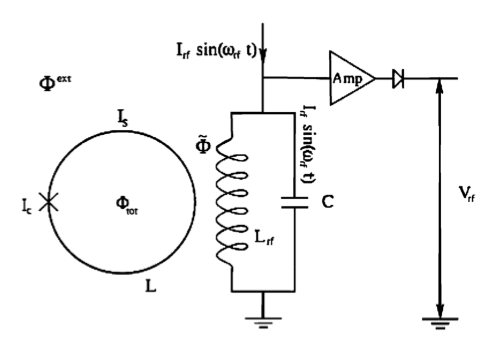
\includegraphics[width = 0.7 \textwidth]{Bilder/SQUID.jpg}
	\caption{Aufbau eines RF-SQUIDs}
\end{figure}

































